% Module 4 section file. Included by ../module4_alfven_continuum_eigenmodes.tex.
\section{Verification, validation, convergence, and sensitivity analysis}
\label{sec:v_and_v}

\subsection{Verification versus validation}
\textbf{Verification} asks whether the equations were solved correctly. \textbf{Validation} asks whether the equations adequately represent the physical system of interest. The present project has substantial verification evidence for the reduced benchmark but no device-level validation of Module 4.

Verification activities include matrix-symmetry tests, analytic scaling tests, decoupled limits, residual checks, grid refinement, regression outputs, and Python/MATLAB parity. Validation would require comparison with experimental measurements or with trusted full-geometry eigenmode calculations using the same equilibrium and physical assumptions.

\subsection{Matrix symmetry}
The Python test checks
\begin{equation}
\frac{\|\mathbf A-\mathbf A^{\mathsf T}\|_F}{\|\mathbf A\|_F}<10^{-12},
\label{eq:symmetry_test}
\end{equation}
where $\|\cdot\|_F$ is the Frobenius norm. This test is sensitive to mismatched face coefficients, asymmetric block assembly, or an inconsistent boundary stencil.

Symmetry is necessary for the intended self-adjoint benchmark, but it is not sufficient for correctness. A symmetrically wrong matrix can still pass Eq.~\eqref{eq:symmetry_test}.

\subsection{Positive spectrum}
All requested baseline eigenvalues satisfy $\omega_j^2>0$. This is consistent with positive $D$ and locally positive-definite harmonic matrices. A stronger test could attempt a sparse Cholesky factorization or estimate the smallest eigenvalue over a broader parameter domain.

\subsection{Decoupled limit}
Set $\epsilon_c=0$. Then $\mathbf C=0$ and
\begin{equation}
\mathbf A=
\begin{bmatrix}
\mathbf K+\mathbf W_m&0\\
0&\mathbf K+\mathbf W_{m+1}
\end{bmatrix}.
\end{equation}
The global problem splits into two independent scalar eigenproblems. Locally,
\begin{equation}
\Omega_-=\min(\omega_m,\omega_{m+1}),
\qquad
\Omega_+=\max(\omega_m,\omega_{m+1}).
\end{equation}
The automated test verifies both the block structure and the local reduction. This is an important physics limit because the coupling mechanism should disappear exactly, not merely become small.

\subsection{Exact Alfv\'en scaling tests}
The tests verify:
\begin{align}
B_0\rightarrow2B_0&\quad\Rightarrow\quad f_j\rightarrow2f_j,\\
\rho(s)\rightarrow4\rho(s)&\quad\Rightarrow\quad f_j\rightarrow\frac{1}{2}f_j.
\end{align}
These transformations probe the diagonal continuum terms, the coupling, and the radial stiffness simultaneously. Failure would reveal inconsistent dimensional construction.

\subsection{Grid-refinement results}
Table~\ref{tab:grid_refinement_textbook} uses the 512-cell solution as an internal comparison rather than an exact value.

\begin{table}[htbp]
\centering
\begin{tabular}{r r r r r}
\toprule
$N$ & Mode 1 (kHz) & Relative error & Mode 2 (kHz) & Relative error\\
\midrule
64  & 160.475766 & $1.871\times10^{-4}$ & 271.034133 & $3.240\times10^{-4}$\\
128 & 160.498664 & $4.447\times10^{-5}$ & 271.101167 & $7.678\times10^{-5}$\\
256 & 160.504376 & $8.887\times10^{-6}$ & 271.117830 & $1.532\times10^{-5}$\\
512 & 160.505802 & 0 & 271.121985 & 0\\
\bottomrule
\end{tabular}
\caption{Grid refinement for the first two frequencies. Errors are relative to the 512-cell values.}
\label{tab:grid_refinement_textbook}
\end{table}

\begin{figure}[htbp]
\centering
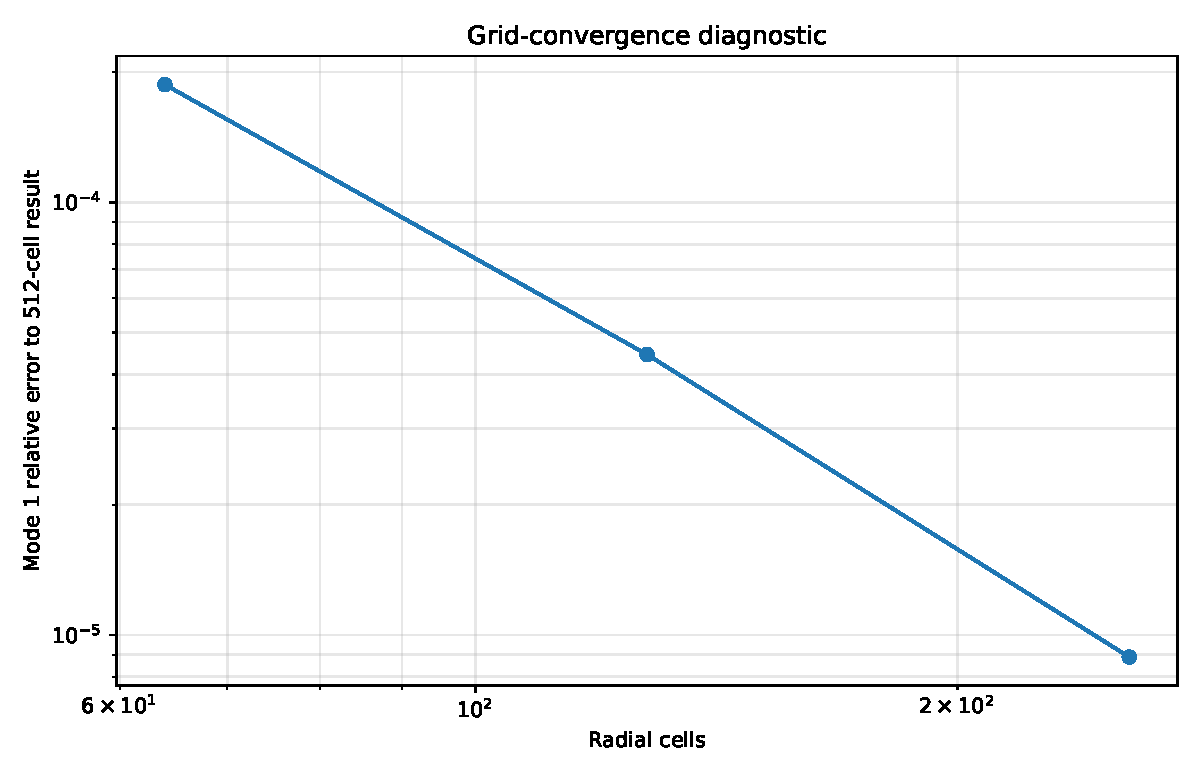
\includegraphics[width=0.82\textwidth]{figures/module4_reduced_ae_convergence.pdf}
\caption{Mode-1 frequency error relative to the 512-cell result. The trend is consistent with approximately second-order spatial behavior over the shown range.}
\label{fig:convergence_textbook}
\end{figure}

An observed order based on three grids can be estimated by
\begin{equation}
p_{\mathrm{obs}}\approx
\frac{\ln\left[(f_h-f_{h/2})/(f_{h/2}-f_{h/4})\right]}{\ln2},
\label{eq:observed_order}
\end{equation}
provided the errors have a consistent sign and the grids are in the asymptotic regime. A more rigorous study should include additional grids and Richardson extrapolation rather than treating the finest grid as exact.

\subsection{Richardson extrapolation}
If
\begin{equation}
f_h=f_*+Ch^p+O(h^{p+1}),
\end{equation}
then two successive grids with refinement ratio $r=2$ give
\begin{equation}
f_*\approx f_{h/2}+\frac{f_{h/2}-f_h}{2^p-1}.
\label{eq:richardson}
\end{equation}
This estimate separates discretization error from the arbitrary choice of finest reference. It should be added when the benchmark is promoted from a regression target to a quantified numerical standard.

\subsection{Python/MATLAB parity}
When MATLAB is available, the test criterion is
\begin{equation}
\max_j\frac{|f_j^{\mathrm{MATLAB}}-f_j^{\mathrm{Python}}|}
{f_j^{\mathrm{Python}}}<10^{-5}.
\label{eq:python_matlab_parity}
\end{equation}
The comparison also uses sign-invariant eigenvector correlation. Agreement between independently written codes reduces the likelihood of language-specific implementation error. It does not prove that both codes did not implement the same mistaken equation or interpretation.

\subsection{Regression testing}
Frozen reference outputs detect unintended changes. The Python regression tolerance for eigenfrequencies is $10^{-10}$ relative. A regression failure can result from a real defect, an intentional model change, a dependency change, or different eigensolver behavior. The appropriate response is investigation and versioning, not automatic replacement of reference data.

\subsection{Sensitivity to coupling strength}
From Eq.~\eqref{eq:gap_at_crossing_omega2}, increasing $|C|$ widens the local gap in squared frequency. Because $C\propto\epsilon_c$, the small-coupling frequency gap is approximately linear in $\epsilon_c$. Global eigenfrequencies need not shift linearly because radial envelopes and harmonic mixing change simultaneously.

A recommended scan is
\begin{equation}
\epsilon_c\in\{0,0.1,0.2,0.3,0.45,0.6,0.8\},
\end{equation}
with mode tracking by overlap. Quantities to record include local gap width, each eigenfrequency, harmonic weights, radial centroid, and overlap with the previous scan point.

\subsection{Sensitivity to radial stiffness}
Increasing $\epsilon_r$ strengthens radial coupling. Recommended diagnostics are:
\begin{equation}
\epsilon_r\in[10^{-4},10^{-2}].
\end{equation}
At very small $\epsilon_r$, envelopes may become narrow and require finer grids. At large $\epsilon_r$, boundary conditions can dominate and modes broaden across the domain. A convincing gap-localized benchmark should exhibit a parameter range in which localization near $s_c$ persists under grid refinement rather than appearing only at one tuned value.

\subsection{Sensitivity to equilibrium profiles}
The crossing position depends on $\iota_0$, $\iota_1$, and $a_\iota$. The frequency scale depends on density. Profile scans should distinguish:
\begin{itemize}[leftmargin=1.6em]
\item rigid dimensional scaling, such as multiplying all density by one factor;
\item shape changes, such as changing $a_\rho$;
\item crossing motion, such as changing $\iota_0$ or $\iota_1$;
\item loss of the crossing from the domain when $\iota_c$ falls outside the profile range.
\end{itemize}

\subsection{Additional verification tests recommended}
The next verification layer should include:
\begin{enumerate}[leftmargin=1.6em]
\item a constant-$D$, constant-potential scalar problem with an analytic mixed-boundary spectrum;
\item manufactured two-component eigenfunctions with a constructed forcing or operator coefficient;
\item discrete orthogonality checks;
\item nonuniform-grid finite-volume convergence;
\item subspace comparison for clustered modes;
\item conservation of the discrete quadratic form in a corresponding time-domain solver;
\item parameter-domain positivity tests.
\end{enumerate}

\subsection{Validation path}
A realistic validation ladder is:
\begin{enumerate}[leftmargin=1.6em]
\item compare the reduced operator with an independently derived cylindrical or large-aspect-ratio TAE model;
\item import a known axisymmetric equilibrium and compare continuum/gap estimates with a trusted code;
\item extend to a three-dimensional stellarator harmonic set and compare with a code such as CAS3D or another suitable eigenmode solver;
\item compare mode frequencies and structures with experimental diagnostics where equilibrium and density uncertainties are quantified.
\end{enumerate}
The present note stops at the verified first rung: a transparent reduced operator.
